\chapter{\chImplementation}
\label{ch:implementation}

\section{System Design}

This section discusses the design of \OurBenchmarkingTool~and the rationale behind the design decisions.

\subsection{Architecture}
\label{sec:impl.architecture}

\begin{figure}
    \centering
    \ifdraft{
        \dummyfig{assets/diagrams/arch.tikz}
    }{
        \makeatletter
\tikzset{
    database/.style={
        path picture={
            \draw (0, 1.5*\database@segmentheight) circle [x radius=\database@radius,y radius=\database@aspectratio*\database@radius];
            \draw (-\database@radius, 0.5*\database@segmentheight) arc [start angle=180,end angle=360,x radius=\database@radius, y radius=\database@aspectratio*\database@radius];
            \draw (-\database@radius,-0.5*\database@segmentheight) arc [start angle=180,end angle=360,x radius=\database@radius, y radius=\database@aspectratio*\database@radius];
            \draw (-\database@radius,1.5*\database@segmentheight) -- ++(0,-3*\database@segmentheight) arc [start angle=180,end angle=360,x radius=\database@radius, y radius=\database@aspectratio*\database@radius] -- ++(0,3*\database@segmentheight);
        },
        minimum width=2*\database@radius + \pgflinewidth,
        minimum height=3*\database@segmentheight + 2*\database@aspectratio*\database@radius + \pgflinewidth,
    },
    database segment height/.store in=\database@segmentheight,
    database radius/.store in=\database@radius,
    database aspect ratio/.store in=\database@aspectratio,
    database segment height=0.1cm,
    database radius=0.25cm,
    database aspect ratio=0.35,
}
\makeatother

\tikzstyle {block} = [draw, text width=4cm, minimum height=1cm, align=center]
\tikzstyle {miniblock} = [draw=gray, dashed, text width=3cm, inner sep=1ex]

\begin{tikzpicture}
    \node [block] (bootstrapper) {Bootstrapper};
    \node [block, below=of bootstrapper] (manager) {Manager};
    \node [block, below=1.5cm of manager, inner sep=0pt] (worker) {
        \begin{tikzpicture}
            \matrix [row sep=1em] {
                \node {Worker}; \\
                \node [miniblock] {\footnotesize Collect System Info}; \\
                \node [miniblock] {\footnotesize Execute run}; \\
                \node [miniblock] {\footnotesize Validate result}; \\
                \node {\dots}; \\
            };
        \end{tikzpicture}
    };
    \draw [-latex'] (manager) -- (worker) node [midway, fill=white] {manages};

    \node [block, right=3cm of bootstrapper] (server) {Server};
    \node[database,database radius=0.5cm,database segment height=0.3cm, below=of server] (database) {};
    \node [right=0.1cm of database] {\rotatebox{-90}{Database}};
    \node [block, below=of database, inner sep=0pt] (analyzer) {
        \begin{tikzpicture}
            \matrix [row sep=1em] {
                \node {Analyzer}; \\
                \node [miniblock] {\footnotesize Summarize runtime}; \\
                \node [miniblock] {\footnotesize Cactus plot}; \\
                \node {\dots}; \\
            };
        \end{tikzpicture}
    };
    \draw (server) -- (database);
    \draw (database) -- (analyzer);

    \draw [-latex'] (bootstrapper) -- (server) node [midway, fill=white] {$R \in C \times I$};
    \path [-latex', transform canvas={xshift=-0.1cm}] (server) edge node [sloped, above, pos=0.33, fill=white] {$(c,i) \in R$} (worker);
    \path [-latex', transform canvas={xshift=0.1cm}] (worker) edge node [sloped, below, pos=0.33, fill=white] {reports to} (server);

    \begin{scope}[on background layer]
        \node[draw=red!50, dashed, inner sep=1ex, label=above:\sffamily\textsc{client-side},  rounded corners, fit=(bootstrapper)(manager)(worker)] (clientenv) {};
        \node[draw=blue!50, dashed, inner sep=1ex, label=above:\sffamily\textsc{server-side},  rounded corners, fit=(server)(database)(analyzer)] (serverenv) {};
        \path [draw=black!30, dashed] ([xshift=1.5cm] clientenv.north east) edge node [sloped, near end, text=black!60, fill=white] {TCP} ([xshift=1.5cm] clientenv.south east);
    \end{scope}

\end{tikzpicture}

    }
    \caption{Architecture of \OurBenchmarkingTool}
    \label{fig:architecture}
\end{figure}

Figure \ref{fig:architecture} shows the architecture of \OurBenchmarkingTool, our attempt on a new benchmarking tool fulfilling most of the defined requirements.
The architecture follows the client-server design pattern, communicating through Transmission Control Protocol (TCP).
The client manages the heavy computation while the server manages the data.
Typically, the client will be in a high performance computing (HPC) cluster system while the server in a separate system---e.g. a virtual private server (VPS)---to avoid long running jobs.

\emph{Server} manages the data in the database.
It receives events through a TCP socket and optionally send replies.
To achieve extensibility, the server maintains a specified set of \emph{observers}, each listening for related events.
The events are distributed through a publisher-subscriber design pattern.
The observer will then executes its jobs, such as inserting data to the database.

\emph{Bootstrapper} is a component that will read the configuration file from the user, prepare the computing environment, and then tell the server $R \in C \times I$, the set of benchmark runs that will be executed.
Among the things prepared are the tools, benchmark instances, and database schema.
Preparing the specified tools and instances may additionally include downloading and running related setting up steps.

\emph{Manager} manages the benchmark workers.
This component acts as an interface to the underlying job submitting system, or even implements its own job queue as in the case of the \emph{local} manager.
The manager is responsible for deploying, assigning tasks, and stopping the benchmark workers, making sure they finishes the assigned job.

\emph{Workers} do the heavy computing steps, typically in parallel.
Because the benchmark run is embarrassingly parallel\footnote{there is no effort needed to parallelize the problem since there is no dependencies between tasks}, each worker can be run as its own process without interacting with other workers.
Submitted to a HPC cluster, this allows the computation to be executed as fast as possible.
A worker is assigned a run identifier and executes the needed steps for the benchmark run after asking the context (i.e. $r = (c, i) \in R$) from the server.
A worker consists of smaller building blocks called \emph{run steps}.
The run step is executed in sequence.
In most cases, one of these steps, called the \emph{executor}, acts as a resource monitor and executes the tool configuration $c$ with the instance $i$.
The executor then measures and limits the execution of the tool.
Finally, each step can report its result to the server.

\emph{Analyzer} aggregates the data from the database and analyze it, outputting a presentable result.
This component is usually used after the benchmarking is finished, but it can also be used to serve a live analysis of a benchmarking in process.
Analyzer also consists of steps that is implemented as a modular, reusable module.
This is to encourage code reuse and minimize the effort of doing the common analysis of research results.


\subsection{Messaging}

\begin{figure}
    \ifdraft{
        \dummyfig{assets/diagrams/zeromq.tikz}
    }{
        \usetikzlibrary{shapes,arrows,positioning,fit,backgrounds}

\tikzstyle{bidirectional} = [draw, latex'-latex', line width=1.15pt]

\tikzset{
    pics/zmq2/.style n args = {3}{
        code = {
        \node[fill=white, minimum height=3em, align=center, text width=9em] (-A) at (0,0) {#1};
        \node[fill=black!5, anchor=north east, text width=4em, align=center] (-B) at (-A.south) {\textsc{#2}};
        \node[fill=black!5, anchor=north west, text width=4em, align=center] (-C) at (-A.south) {\textsc{#3}};
        \node[inner sep=0pt,draw,rounded corners,fit=(-A)(-B)(-C)] {};
        \draw (-B.north west) -- (-C.north east)
              (-B.north east) -- (-C.south west);
        }
    },
    pics/zmq1/.style n args = {2}{
        code = {
        \node[fill=white, minimum height=3em, align=center, text width=5em] (-A) at (0,0) {#1};
        \node[fill=black!5, anchor=north, text width=5em, align=center] (-B) at (-A.south) {\textsc{#2}};
        \draw (-B.north west) -- (-B.north east);
        \node[inner sep=0pt,draw,rounded corners,fit=(-A)(-B)] {};
        }
    },
}


\resizebox{\textwidth}{!}{%
    \begin{tikzpicture}
        \node (workerdots) {\huge\vdots};
        \pic [above=of workerdots, local bounding box=worker2] (w2) {zmq1={Worker 2}{dealer}};
        \pic [above=2cm of worker2, local bounding box=worker1] (w1) {zmq1={Worker 1}{dealer}};
        \pic [below=of workerdots, local bounding box=workern] (wn) {zmq1={Worker $n$}{dealer}};

        \pic [right=3cm of workerdots, local bounding box=server] (s) {zmq2={Gateway}{router}{pub}};

        \node [right=3cm of server] (observerdots) {\huge\vdots};
        \pic [above=of observerdots, local bounding box=observer2] (o2) {zmq1={Observer 2}{sub}};
        \pic [above=of observer2, local bounding box=observer1] (o1) {zmq1={Observer 1}{sub}};
        \pic [below=of observerdots, local bounding box=observern] (on) {zmq1={Observer $n$}{sub}};

        \draw [bidirectional] (w1-B.east) -- (s-B.west);
        \draw [bidirectional] (w2-B.east) -- (s-B.west);
        \draw [bidirectional] (wn-B.east) -- (s-B.west);

        \draw [bidirectional] (s-C.east) -- (o1-B.west);
        \draw [bidirectional] (s-C.east) -- (o2-B.west);
        \draw [bidirectional] (s-C.east) -- (on-B.west);

        \node [inner sep=.5cm, text=red!60!black, above, rotate=90, text width=4em] (w1label) at (worker1.west) {\sffamily\textsc{worker process}};
        \node [inner sep=.5cm, text=red!60!black, above, rotate=90, text width=4em] (w2label) at (worker2.west) {\sffamily\textsc{worker process}};
        \node [inner sep=.5cm, text=red!60!black, above, rotate=90, text width=4em] (wnlabel) at (workern.west) {\sffamily\textsc{worker process}};


        \begin{scope}[on background layer]
            \node[fit=(worker1)(worker2)(workerdots)(workern)] (workers) {};
            \node[fit=(observer1)(observer2)(observerdots)(observern)] (observers) {};

            \node[fill=red!5, rounded corners, fit=(worker1)(w1label)] {};
            \node[fill=red!5, rounded corners, fit=(worker2)(w2label)] {};
            \node[fill=red!5, rounded corners, fit=(workern)(wnlabel)] {};
            \node[fill=blue!5, rounded corners, fit=(server)(observers)] (serverenv) {};
        \end{scope}

        \node [inner sep=.5cm, text=blue!60!black, below right] at (serverenv.north west) {\sffamily\textsc{server process}};


    \end{tikzpicture}
}
    }
    \caption{Messaging architecture of \OurBenchmarkingTool}
    \label{fig:zmq}
\end{figure}

Figure \ref{fig:zmq} gives an overview of the messaging architecture and the overall network of \OurBenchmarkingTool.
Each process is independent to each other and can be separated across virtual nodes.
This means it can be implemented in a single node, in a cluster system, or even across clusters.
Data is transported through TCP for inter-process communication, and through local in-process (inter-thread) transportation for intra-process communication.
Communication follows some basic messaging patterns used by the \O{}MQ (ZeroMQ) messaging framework, namely \textsc{router-dealer} and \textsc{pub-sub}.

The \textsc{router-dealer} patterns allows two-way communication between the party \citep{hintjens2013zeromq}.
This is used in the communication between the worker and the server gateway.
The patterns allows many workers to send events to the server and optionally request for a reply from the server.
The message sent to a \textsc{router} socket is enveloped by a unique identifier, allowing the \textsc{router} to reply to the correct \textsc{dealer}.
This powerful pattern allows reliable many to one communication between the workers and the server gateway.

On the other hand, \textsc{pub-sub} patterns follows the publisher-subscriber pattern as its name suggests \citep{hintjens2013zeromq}.
This is a fan-out pattern, on which the publisher just publish the message without caring if the message is received.
Both the publisher and subscriber does not know each other.
The \textsc{pub} socket just publish the message to the socket, and the \textsc{sub} sockets listen to one or more `topic'.
This allows fast distribution of event message received by the server gateway to the possibly many observers.
The downside is the distribution is not reliable since the message is just thrown without confirmation if the other party is ready.
This can be corrected with proper synchronization using other messaging pattern if needed.


\subsection{Benchmarking Workflow}
\begin{figure}
    \centering
    \ifdraft{
        \dummyfig{assets/pics/workflow-swimlane.png}
    }{
        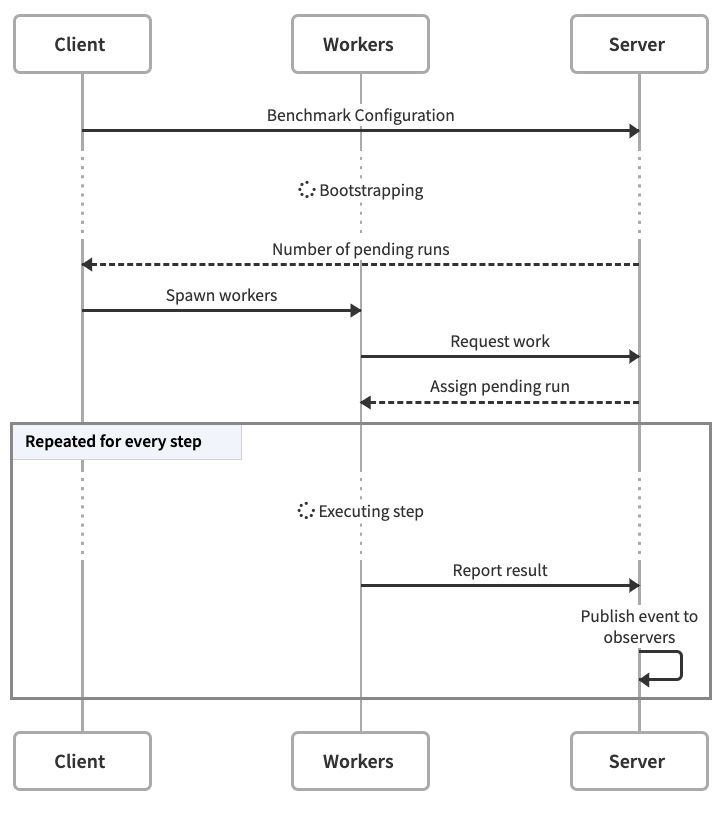
\includegraphics[width=\textwidth]{assets/pics/workflow-swimlane.png}
    }
    \caption{Benchmarking workflow}
    \label{fig:swimlane}
\end{figure}

Figure \ref{fig:swimlane} presents the steps and interactions taken by each actors, namely the Client, Workers, and Server.
Aside from the already defined Workers and Server in Section \ref{sec:impl.architecture} above, Client represents the actual user interfacing with \OurBenchmarkingTool.

% ...

As soon as soon as the bootstrapping is done, analysis can be executed from the available data in database.
This allows the flexibility of doing either on-demand analysis or live analysis.


\subsection{Benchmarking Model}

% TODO: ER Diagram


\subsection{Design Rationale}


\section{Implementation}
\section{Usage Scenario}
